\documentclass[10pt,a4paper]{article}

\usepackage{graphicx}
\usepackage[left=2.5cm,right=2.5cm,top=2.5cm,bottom=2.5cm]{geometry}
\usepackage{geometry}
\usepackage{pdflscape}


\begin{document}
\title{Work Plan for the Selection of the $\mu$Reactor Design at UIUC\\}
\author{Draft\\ \\ \\ \\ Kathryn D. Huff,\\
Mehmet Turkmen,\\
Zoe Richter}
\date{\today}
\maketitle

\pagebreak
\section{Introduction}
Micro-reactors are the reactors which produce power typically less than 20 MWe and site less than 500 m2 (0.1 acre) in the size of shipping container or a big house. They are considered to be automated operation with minimum operating staff. Due to the small size and low consequences of micro-reactors, the regulations applied to the existing (non)commercial reactors may not fully applicable to micro-reactors. Apart from other advanced reactor designs like SMRs, micro-reactors have specific following licencing issues: security, aircraft strike, emergency preparedness, source term analysis, staffing, remote operation, decommissioning, transportation, manufacturing licenses, quality assurance, probabilistic risk assessment and NRC oversight.

\section{Reactors}
Six reactors are under investigation: eVinci, Holosgen, MicroNuclear, NuScale, Oklo, Starcore, Urenco and X-energy (in alphabetical order). Kairos does not have any μReactor designs which produce power less than 200 MWe. A comparison of reactors under consideration is listed in Table 1. The design reviews around the world have given in Table 2. 

\pagebreak
\newgeometry{margin=1cm}
\begin{landscape}
\begin{table} [ht]
\begin{center}

\caption{A brief comparison of micro-reactor designs (\cite{Yan20};\cite{Arafat19};\cite{Levinsky18};\cite{IAEA18})}
\begin{tabular}{|l|l|l|l|l|l|l|l|l|}
\hline 
Design 		&eVinci 		& Holos (Zoe)		&MegaPower 	& NuScale		& Oklo 		& Starcore		& Urenco 		& Xe-100 \\ 
\hline 
Institution 	&Westinghouse& Holosgen	&MegaPower	& NuScale		& Oklo Inc. 	& Starcore		& Urenco 		& X-energy \\ 
\hline 
Type			&Heat Pipe	&   		  	& PWR 		& Heat Pipe	&   			&			&   			& HTGR (Pebble)\\ 
\hline 
Spectrum		&Epithermal	&  		 	& Thermal 	& Fast		&   			&   			&			&Thermal\\ 
\hline 
Power (MWe)	&0.2-5		&   			&			& 50 			&   			&   			&			&75\\ 
\hline
Refueling (years)&5 to 10		&   			&			& 2 			&   			&   			&			&Online refueling\\ 
\hline
Enrichment (\%)&19.75		&   			&			& {<} 4.95 		&   			&   			&			&15.5\\ 
\hline
Core Height / Diameter (m)	&/ 1.5		&   			&			& / 1.5 		&   			&   			&			&23 / 5\\ 
\hline
Fuel			&UN/U-Mo	&   			&			&UO2 (NuFuel HTP2)		&   			&   			&			&UCO TRISO\\ 
\hline
Clad			&-		&   			&			& M5 		&   			&   			&			&-\\ 
\hline
Heat Pipe fluid	&Na/K	&   			&			& - 		&   			&   			&			&-\\ 
\hline
\end{tabular}

\caption{Worldwide design reviews}
\begin{tabular}{|l|l|l|l|l|l|}
\hline 
	 &Country of Origin 	& Company		&Reactor type			&Output(MWe) 	& Status \\ 
\hline 
1 	&Canada/US		& Terrestrial Energy	&Molten Salt Integral	&200		& PHASE 1 COMPLETED \\ 
 	&		& 	&	&		& PHASE 2 PENDING  \\
\hline 
2 	&US/Korea/China	& UltraSafe Nuclear	&High-temperature gas prismatic block	&5		& PHASE 1 IN PROGRESS completion date 2018   \\ 
 	&		& /Global First Power	&	&		& PHASE 2 Service Agreement under development  \\
\hline
3 	&Sweden/Canada	&LeadCold	&Molten lead pool fast spectrum	&3-10		& PHASE 1 ON HOLD AT VENDOR REQUEST  \\ 
\hline
4 	&US		&Advanced Reactor Concepts	&Sodium pool fast spectrum	&100		& PHASE 1 IN PROGRESS  \\ 
\hline
5 	&UK		&U-Battery	&High temperature gas prismatic block	&4		& PHASE 1 Service Agreement under development  \\ 
\hline
6 	&UK		&Moltex Energy	&Molten salt fast spectrum	&300		& PHASE 1 IN PROGRESS  \\ 
\hline
7 	&Canada/US		&StarCore Nuclear	&High-temperature gas prismatic block	&10		& PHASE 1 and 2 Service Agreement under development   \\ 
\hline
8 	&US		&SMR, LLC. &Pressurized Water	&160		&PHASE 1 Service Agreement under development   \\ 
 	&		& (A Holtec International Company)		&	&		&  \\
\hline
9 	&US		&NuScale Power	&Integral Pressurized Water	&50		&PHASE 2* Service Agreement under development   \\ 
\hline
10 	&US		&Westinghouse Electric Co.	&eVinci Micro Reactor	&<25		&PHASE 2* Service Agreement under development  \\ 
\hline
11 	&Japan		&4S	&Na cooled fast reactor	&10		&Licensing pre-application  \\ 
\hline
12 	&Russia		&ABV	&PWR	&2x7.9		&Part of design licensed  \\ 
\hline
13 	&Argentina	&CAREM-25	&PWR	&27		&Licensing in progress  \\ 
\hline
14 	&Russia		&KLT-40S	&PWR	&2x35	&Licensed and under construction  \\ 
\hline
\end{tabular}

\end{center}
\end{table}
\end{landscape}
\restoregeometry


\subsection{eVinci - Westinghouse}
Full design details have not been revealed yet for the public; only general information is given by the company. However, several academic studies, most of them eVinci-like, can be found in the literature. Recently, two papers, \cite{Xu19} and \cite{Wright19}, have been published in 18th NURETH conference. Those are not available for now but reaching them somehow would be valuable. Westinghouse is planning to finalize the current design of eVinci by 2022, testing by 2023 and commercializing by 2025. Hernandez et al. \cite{Hernandez19} performed a series of calculations in eVinci-like (not eVinci) for natural resource utilization, burnup analyses, waste management and environmental impacts. The details of eVinci design obtained from the documents published by Westinghouse are presented in Table 3. 

\begin{table} [ht]
\begin{center}

\caption{eVinci design parameters}
\begin{tabular}{|l|l|l|}
\hline 
Design 		&Value (from Westinghouse reports) 		& Value (other)\\ 
\hline 
Core Diameter (in) 		&59.06 		&  \\ 
\hline 
Monolith materials 		& 		& Type-316 SS	\\ 
\hline 
Refueling (years) 		&Up to 10 		&  \\ 
\hline 
Fuel 		&UN/U-Mo 		& 	 \\ 
\hline 
Fuel Pellet Density, \% TD 		&96 		&  \\ 
\hline 
Enrichment (\%) 		&19.75 		&  \\ 
\hline 
Fuel channel radius (in) 		& 		& 0.281 \\ 
\hline 
Number of fuel channels 		&378 (1 MWth), 4219 (14 MWth)		& 2112 (5 MWth) \\ 
\hline 
Reflector material 		&		& BeO\\ 
\hline 
HP channel radius (in) 		&		& 0.298\\ 
\hline 
Number of HP channels 		& 		& 1224\\ 
\hline 
HP to HP web thickness (in) 		& 		& 0.039\\ 
\hline 
Fuel to fuel web thickness (in) 		& 		& 0.059\\ 
\hline 
HP total length (ft) 		&		& 13.12\\ 
\hline 
HP fluid 		&Na/K		& \\ 
\hline 
HP fluid temperature (K) 		&920 		& \\ 
\hline

\end{tabular}
\end{center}
\end{table}

\begin{figure}[hbtp]
\centering
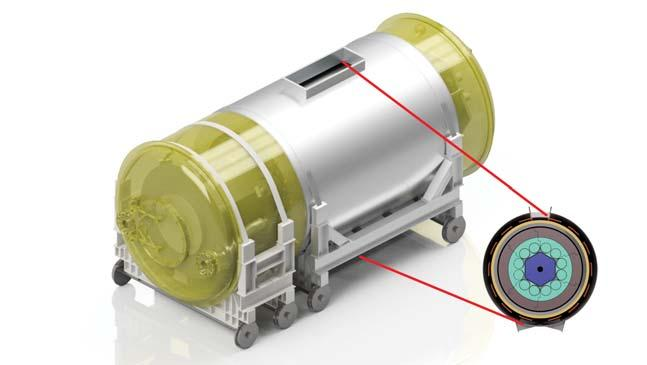
\includegraphics[scale=0.5]{fig1.jpeg}
\caption{eVinci Core Configuration}
\end{figure}

\begin{figure}[hbtp]
\centering
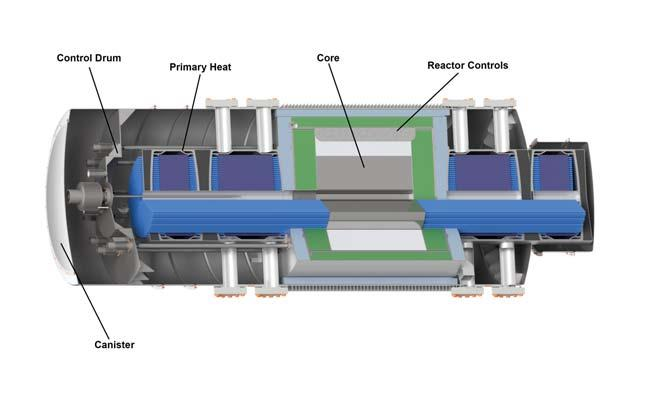
\includegraphics[scale=0.5]{fig2.jpeg}
\caption{eVinci Micro Reactor Overview}
\end{figure}


\subsection{Holosgen}

\subsection{MicroNuclear}
There is absolutely nothing on MsNB design of MicroNuclear LLC company. I think this company has a weak desire to get into the micro-nuclear world. Maybe they are only showing an interest on the μR. 

\subsection{MegaPower}

\subsection{NuScale}
Detailed technical specifications (as seen in Table 4) related to reactor core design, source term, licensing requirements and safety assessments are given in the NRC web-page \cite{NuScale18}. This is the FSAR for the SMR design of NuScale. NuScale considers two different micro-reactor concepts: the one (10-50 MWe) based on current small modular reactor tecnhnology and the other one (10-50 MWe) based on heat pipe reactor technology. The first one is very similar to the SMR. FSAR report  seems quite sufficient by supplying all the details about the plant. This design can be altered for the μR concept of NuScale for a nominal electric power of less than 20 MW.

\begin{table} [ht]
\begin{center}

\caption{NuScale Reactor Core Description (\cite{NuScale18}}
\begin{tabular}{|l|l|}
\hline 
Design 		&Value \\ 
\hline 

\end{tabular}
\end{center}
\end{table}

\begin{figure}[hbtp]
\centering
\includegraphics[scale=0.5]{}
\caption{NuScale MCNP view (radial)}
\end{figure}

\begin{figure}[hbtp]
\centering
\includegraphics[scale=0.5]{}
\caption{NuScale Reactor Overview}
\end{figure}

\subsection{Oklo}

\subsection{Starcore}

\subsection{Urenco}

\subsection{X-energy}

\begin{table} [ht]
\begin{center}

\caption{ X-energy design}
\begin{tabular}{|l|l|}
\hline 
Design 		&Value \\ 
\hline 
Core Diameter (m) 		&4.88 \\ 
\hline 
Core Height (m) 		&20 \\ 
\hline 
Refueling		&Online fuel loading 
175 fresh pebbles/day \\ 
\hline 
Fuel		&UCO TRISO Pebbles \\ 
\hline 
Enrichment (\%)		&15.5 \\ 
\hline 
Number of fuel pebbles		&220,000 \\ 
\hline 
Number of TRISO particles per pebble		&18,000 \\ 
\hline 
Pebble fuel core diameter (mm)		&55 \\ 
\hline 
Pebble diameter (mm)	&55 \\ 
\hline 
Pebble fuel core diameter (mm)		&60 \\ 
\hline 
Number of passes		&60\\ 
\hline 
Final burnup (GWd/tHM)		&160 \\ 
\hline 
Burnable poison		&no \\ 
\hline 
Power density (MW/m3)		&4.8 \\ 
\hline 
UCO TRISO kernel radius (mm)	&0.2125 \\ 
\hline 
Porous Carbon Buffer thickness (mm)	&0.095 \\ 
\hline 
Inner Pyrolytic Carbon Layer thickness (mm) 	&0.04 \\ 
\hline 
Silicon Carbide Layer thickness (mm)	&0.035 \\ 
\hline 
Outer Pyrolytic Carbon Layer thickness (mm)	&0.04 \\ 
\hline 
Core Inlet temp (C)	&259 \\ 
\hline 
Core Outlet temp (C) 	&750 \\ 
\hline 
Core Inlet Pressure (MPa)	&6 \\ 
\hline 
Core Outlet Pressure (MPa)	&5.84 \\ 
\hline 

\end{tabular}
\end{center}
\end{table}

\begin{figure}[hbtp]
\centering
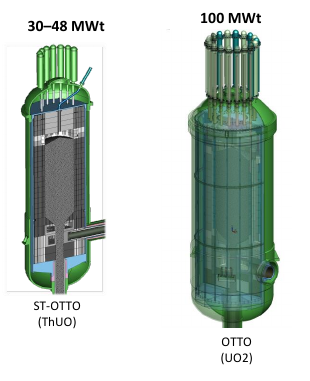
\includegraphics[scale=1]{fig5.jpeg}
\caption{X-energy micro-reactor overview}
\end{figure}

\section{Site Requirements}
Idaho National Laboratory, “Modernization of Technical Requirements for Licensing of Advanced Non-Light Water Reactors, Probabilistic Risk Assessment Approach,” Rev 0, August 2019.\\ 
Idaho National Laboratory, “Modernization of Technical Requirements for Licensing of Advanced Non-Light Water Reactors, Selection and Evaluation of Licensing Basis Events,” Rev 0, August 2019.\\ 
Idaho National Laboratory, “Modernization of Technical Requirements for Licensing of Advanced Non-Light Water Reactors, Safety Classification and Performance Criteria for Structures, Systems and Components,” Rev 0, August 2019.\\ 
Idaho National Laboratory, “Modernization of Technical Requirements for Licensing of Advanced Non-Light Water Reactors, Risk-Informed and Performance-Based Evaluation of Defense-inDepth Adequacy,” Rev 0, August 2019.


\section{Source Term}
A general source term analysis comprises transient scenario modeling, fuel pin radionuclide distribution, failed pin radionuclide release, radionuclide bubble transport, offsite dispersion analysis and containment region analysis. Some of them can, however, be eliminated or new ones can be added depending on which micro-reactor is to be chosen. As an example, the micro-reactor design does not include any spent fuel storage, thus the source term would not.
For the source term analysis of a selected micro-reactor design, phenomena and release paths of accident scenarios first need to be identified. Pathways for some advanced reactors (i.e., HTGR, SFR, MSR) are illustrated in Fig. 6. There are on-going discussions in the NRC on the evaluation of the source term of micro-reactors; it is expected to come to a conclusion on the licencing issues including the source term by the end of this year (estimated). 

\begin{figure}[hbtp]
\centering
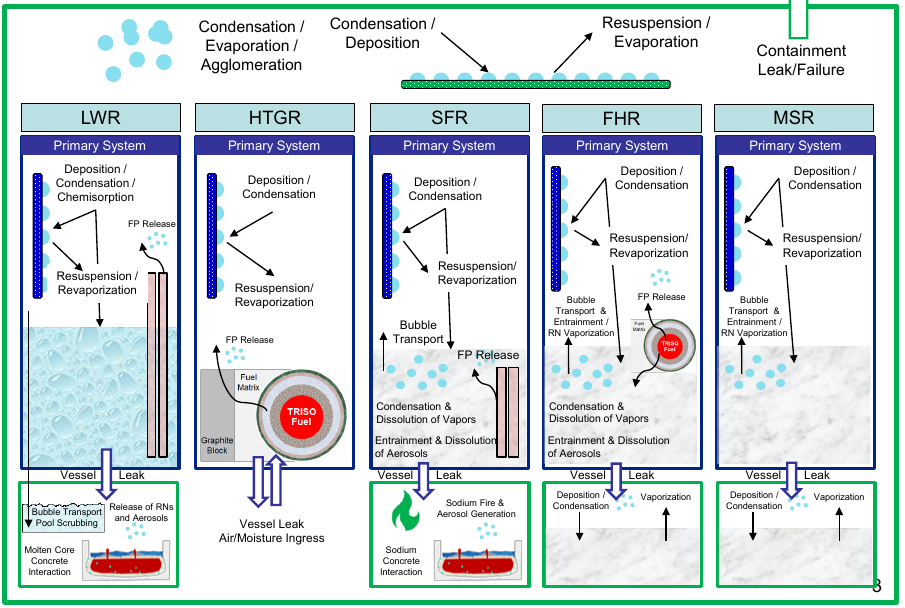
\includegraphics[scale=0.6]{fig6*.jpeg}
\caption{Pathway for radioactive release for several reactor types}
\end{figure}

\begin{figure}[hbtp]
\centering
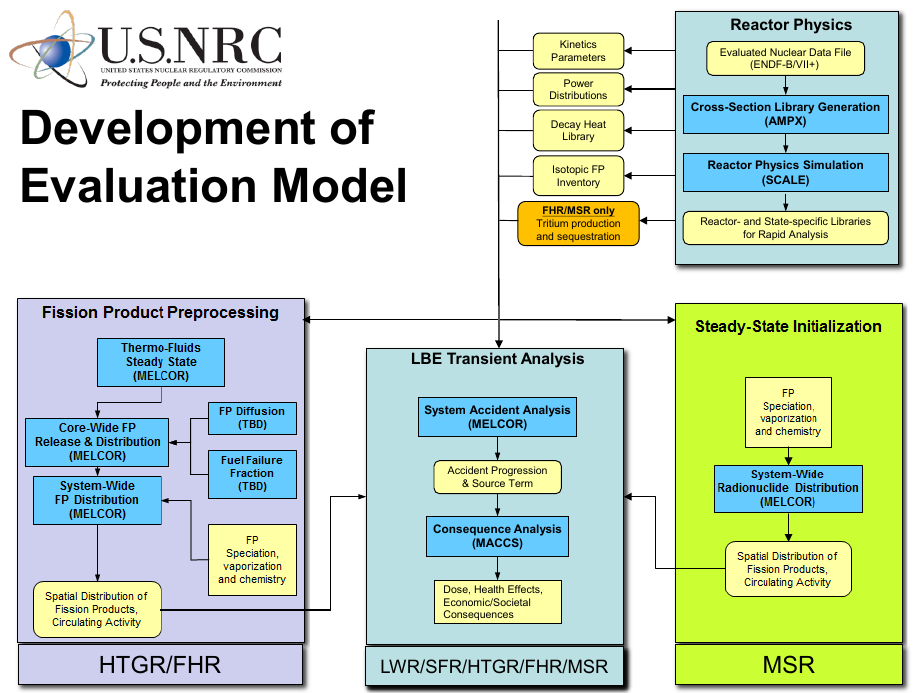
\includegraphics[scale=0.6]{fig7.jpeg}
\caption{Source term evaluation model}
\end{figure}

There is a possibility to make an assumption for the pathway identification of the micro-reactors. We can use the same or modified pathways of the existing reactors, accepted by the NRC, for the analogy to the selected micro-reactor design. Yet, heat pipe reactors may still require as the release ways have not completely known.
The method for the source term calculation recommended by the NRC is given in Fig. 7. The method to be applied changes with the type of the reactor. In any cases, MELCOR, system accident analysis code, produce the source term for the defined design-basis accidents. 
For probabilistic offsite consequence analysis bounded by the calculated source term, MACCS code needs to be utilized. The code is capable of evaluating the Level 3 PRA including the radionuclide release, atmospheric transport, meteorology, protective actions, site data, dosimetry, health effects, economic factors, and so forth. Design-specific and site-related issues must be input to the code.  Meteorological statistics (i.e., day and night temperatures, magnitude and direction of the wind, tornados, flooding level), topographical data and population density and distribution, habitat of the animals and the location of the endemic plants are to be recorded.   
The methodology and the results on the source term calculations are presented in detail in the relevant documents of NuScale \cite{NuScale18} and eVinci \cite{Southern19}.
According to the NuScale, the potential radionuclide source term associated with a severe accident is much smaller (5\%) than that associated with a 1000 MWe design. This value is 1\% for eVinci. 

\section{Licencing Procedure}


\section{Safety Assessment}
This part is going to be discussed later but will include accident scenarios including design-basis that a nuclear facility must be designed and built to withstand, and beyond design accidents that are possible but were not fully considered in the design process.

\section{Discussion on the Report}


\section{Conclusion}


\begin{thebibliography}{X}
\bibitem{Xu19} Hong Xu, Jurie J. van Wyk, Richard F. Wright, “Thermal Analysis for eVinci Micro™ Reactor,” 18th International Topical Meeting on Nuclear Reactor Thermal Hydraulics (NURETH18), August 18-23, 2019. 
\bibitem{Wright19} Richard F. Wright, Andrew M. Dokmanovich, “Phenomena Identification and Ranking Table for the eVinciTM Micro Reactor,” 18th International Topical Meeting on Nuclear Reactor Thermal Hydraulics (NURETH18), August 18-23, 2019. 
\bibitem{Yan20} B.H. Yan, C. Wang, L.G. Li, “The technology of micro heat pipe cooled reactor: A review,” Annals of Nuclear Energy 135 (2020) 106948.
\bibitem{Arafat19} Yasir Arafat, Jurie Van Wyk, “Nuclear Plant Journal: eVinci™ Micro Reactor – Our Next Disruptive Technology,” http://www.westinghousenuclear.com/Portals/0/new%20plants/evincitm/eVinci%20Micro%20Reactor%20NPJ%20M-A%202019.pdf?ver=2019-04-30-211410-367
\bibitem{Hernandez19} Richard Hernandez, Michael Todosow, Nicholas R. Brown, “Micro heat pipe nuclear reactor concepts: Analysis of fuel cycle performance and environmental impacts”, Annals of Nuclear Energy 126 (2019) 419–426.
\bibitem{NuScale19} NuScale, “NuScale Standard Plant Design Certification Application - Chapter 4: Reactor, Part 2-Tier 2”, Revision 2, ML18310A325, October 2018. https://www.nrc.gov/reactors/new-reactors/design-cert/nuscale.html. 
\bibitem{Southern19} Southern Company, “Modernization of Technical Requirements for Licensing of Advanced Non-Light Water Reactors: Westinghouse eVinciTM Micro-Reactor Licensing Modernization Project Demonstration”, DOE, SC-29980-202, 2019.
\bibitem{NuScale18} NuScale, “NuScale Standard Plant Design Certification Application: Chapter Nineteen Probabilistic Risk Assessment and Severe Accident Evaluation”, Rev. 2, 2018. 
\bibitem{Levinsky18} Levinsky, A., Wyk, J.J., Arafat, Y., et al., 2018. Westinghouse eVinci Reactor for Off-Grid Markets. Transactions of the American Nuclear Society, Orlando, Florida, November 11-15.
\bibitem{IAEA18} IAEA, “Advances in Small Modular Reactor Technology Developments A Supplement to: IAEA Advanced Reactors Information System (ARIS)”, 2018. 

\end{thebibliography}

\end{document}